%%%%%%%%%%%%%%%%%%%%%%%%%%%%%%%%%%%%%%%%%
% Beamer Presentation
% LaTeX Template
% Version 1.0 (10/11/12)
%
% This template has been downloaded from:
% http://www.LaTeXTemplates.com
%
% License:
% CC BY-NC-SA 3.0 (http://creativecommons.org/licenses/by-nc-sa/3.0/)
%
%%%%%%%%%%%%%%%%%%%%%%%%%%%%%%%%%%%%%%%%%


%----------------------------------------------------------------------------------------
%	PACKAGES AND THEMES
%----------------------------------------------------------------------------------------

\documentclass{beamer}

\mode<presentation> {

% The Beamer class comes with a number of default slide themes
% which change the colors and layouts of slides. Below this is a list
% of all the themes, uncomment each in turn to see what they look like.

%\usetheme{default}
%\usetheme{AnnArbor}
%\usetheme{Antibes}
%\usetheme{Bergen}
%\usetheme{Berkeley}
%\usetheme{Berlin}
%\usetheme{Boadilla}
%\usetheme{CambridgeUS}
%\usetheme{Copenhagen}
%\usetheme{Darmstadt}
%\usetheme{Dresden}
%\usetheme{Frankfurt}
%\usetheme{Goettingen}
%\usetheme{Hannover}
%\usetheme{Ilmenau}
%\usetheme{JuanLesPins}
%\usetheme{Luebeck}
\usetheme{Madrid}
%\usetheme{Malmoe}
%\usetheme{Marburg}
%\usetheme{Montpellier}
%\usetheme{PaloAlto}
%\usetheme{Pittsburgh}
%\usetheme{Rochester}
%\usetheme{Singapore}
%\usetheme{Szeged}
%\usetheme{Warsaw}

% As well as themes, the Beamer class has a number of color themes
% for any slide theme. Uncomment each of these in turn to see how it
% changes the colors of your current slide theme.

%\usecolortheme{albatross}
%\usecolortheme{beaver}
%\usecolortheme{beetle}
%\usecolortheme{crane}
%\usecolortheme{dolphin}
%\usecolortheme{dove}
%\usecolortheme{fly}
%\usecolortheme{lily}
%\usecolortheme{orchid}
%\usecolortheme{rose}
%\usecolortheme{seagull}
%\usecolortheme{seahorse}
%\usecolortheme{whale}
%\usecolortheme{wolverine}

%\setbeamertemplate{footline} % To remove the footer line in all slides uncomment this line
%\setbeamertemplate{footline}[page number] % To replace the footer line in all slides with a simple slide count uncomment this line

%\setbeamertemplate{navigation symbols}{} % To remove the navigation symbols from the bottom of all slides uncomment this line
}

\usepackage{graphicx} % Allows including images
\usepackage{booktabs} % Allows the use of \toprule, \midrule and \bottomrule in tables
\usepackage{amsmath} % Allows the use of \toprule, \midrule and \bottomrule in tables
\usepackage{xcolor}
\newcommand{\norm}[1]{{\left\lVert#1\right\rVert}}

%----------------------------------------------------------------------------------------
%	TITLE PAGE
%----------------------------------------------------------------------------------------

\title[Metastability for the Contact Process]{Metastability for the Contact Process on Z: Part 2} % The short title appears at the bottom of every slide, the full title is only on the title page

\author{Kacper Urbański} % Your name
\institute[UvA] % Your institution as it will appear on the bottom of every slide, may be shorthand to save space
{
Universiteit van Amsterdam \\ % Your institution for the title page
\medskip
\textit{kacper.urbanski@protonmail.com} % Your email address
}
\date{\today} % Date, can be changed to a custom date

\begin{document}

\begin{frame}
\titlepage % Print the title page as the first slide
\end{frame}

\begin{frame}
\frametitle{Overview} % Table of contents slide, comment this block out to remove it
\tableofcontents % Throughout your presentation, if you choose to use \section{} and \subsection{} commands, these will automatically be printed on this slide as an overview of your presentation
\end{frame}

%----------------------------------------------------------------------------------------
%	PRESENTATION SLIDES
%----------------------------------------------------------------------------------------

%------------------------------------------------
\section{Forumlating the theorem} % Sections can be created in order to organize your presentation into discrete blocks, all sections and subsections are automatically printed in the table of contents as an overview of the talk
%------------------------------------------------

\subsection{Natural language definition} % A subsection can be created just before a set of slides with a common theme to further break down your presentation into chunks

\begin{frame}
    \frametitle{A bit of terminology}
    \begin{itemize}
        \item $\xi$ - 'xi'
        \item $\xi_N$ - 'xi n'
        \item $\xi_{[-N, \infty)}$ - 'xi plus inf'
        \item $\xi_{(-\infty, N]}$ - 'xi minus inf'
        \item $[-N, N]$ - 'main interval'
        \item $\xi_N(t) \ne \varnothing$ - 'process is still alive'
    \end{itemize}
\end{frame}

\begin{frame}
    \frametitle{Natural language definition of metastability}

    Recall that a system is metastable if:
    \begin{enumerate}
        \item It stays out of its equilibrium during a memoryless random time
        \item During this time in which the system is out of equilibrium it stabilizes
    \end{enumerate}
    Let's elaborate some more on point 2.
    \begin{enumerate}
        \item Assume that for a given $N$ we have some intermediate timescale such $R_N$ that $R_N << \beta_N$
        \item Say we measure a temporal mean of some observable quantity of a system (e.g. particle density) over this timescale
        \item We say system has stabilized if this mean is close to the expectation of this observable quantity w.r.t. some fixed probability distribution on $\{0,1\}^{\mathbb{Z}}$
    \end{enumerate}
\end{frame}

\subsection{Towards the rigorous definition} % A subsection can be created just before a set of slides with a common theme to further break down your presentation into chunks

\begin{frame}
    \frametitle{Towards the rigorous definition}
    To ensure $R_N << \beta_N$, let's require $R_N / \beta_N \rightarrow 0$ as $N \rightarrow \infty$.
    \\~\\ 
    For our purposes, define \textbf{observable quantity of a system} as $f(\xi_N(t))$, such that:
    \begin{itemize}
        \item $f : \{0,1\}^{\mathbb{Z}} \rightarrow \mathbb{R}$
        \item $f$ is local
    \end{itemize}
\end{frame}

\begin{frame}
    \frametitle{Towards the rigorous definition}

    Define \textbf{temporal mean} of observable quantity $f(\xi_N(t))$ as:
    \[
        A^N_R(s, f) := R^{-1}\int_s^{s+R}f(\xi_N(t))dt
    \]
    Where:
    \begin{itemize}
        \item $s$ is the time in which we start our measurement
        \item $R$ is the duration over which we calculate the temporal mean
    \end{itemize}
\end{frame}

\begin{frame}
    \frametitle{Towards the rigorous definition}

    Recall what we said about the 2nd condition for metastability:

    \begin{enumerate}
        \item \textcolor{gray}{Assume that for a given $N$ we have some intermediate timescale such $R_N$ that $R_N << \beta_N$
            \item Say we measure a temporal mean of some observable quantity of a system (e.g. particle density) over this timescale
            \item We say system has stabilized if this mean is close to the expectation of this observable quantity w.r.t. some fixed probability distribution on $\{0,1\}^{\mathbb{Z}}$}
    \end{enumerate}
\end{frame}

\begin{frame}
    \frametitle{Towards the rigorous definition}

    Recall what we said about the 2nd condition for metastability:

    \begin{enumerate}
            \item Assume that for a given $N$ we have some intermediate timescale such $R_N$ that $R_N << \beta_N$
            \item Say we measure a temporal mean of some observable quantity of a system (e.g. particle density) over this timescale
            \item \textcolor{gray}{We say system has stabilized if this mean is close to the expectation of this observable quantity w.r.t. some fixed probability distribution on $\{0,1\}^{\mathbb{Z}}$}
    \end{enumerate}
\end{frame}

\begin{frame}
    Take our \textbf{fixed probability distribution} to be $\mu$ (i.e. the non-zero invariant measure of the contact process in the supercritical regime). \\~\\

    Then, we can define \textbf{expectation of observable quantity} w.r.t to this probability distribtuion as $\mu(f) := \int fd\mu$ (I will call this quantity simply ``expectation'').
\end{frame}

\begin{frame}
    Take convergence in probability as how we understand \textbf{closeness}. \\~\\
    Thus, we want to have a sequence $R_N$, such that:
    \begin{itemize}
        \item $R_N / \beta_N \rightarrow 0$ as $N \rightarrow \infty$
        \item for all $\varepsilon > 0$ and all observable quantities $f$
        \[
            \mathbb{P}\left[ |A_{R_N}(s, f) - \mu(f)|\right < \varepsilon] \rightarrow 0
        \]
    \end{itemize}

    As $N \rightarrow \infty$. \\~\\
    Are we done now?
    \textcolor{white}{\textbf{No!} How do we choose $s$ (the starting point of temporal mean measurement)?}
\end{frame}

\begin{frame}
    Take convergence in probability as how we understand \textbf{closeness}. \\~\\
    Thus, we want to have a sequence $R_N$, such that:
    \begin{itemize}
        \item $R_N / \beta_N \rightarrow 0$ as $N \rightarrow \infty$
        \item for all $\varepsilon > 0$ and all observable quantities $f$
        \[
            \mathbb{P}\left[ |A_{R_N}(s, f) - \mu(f)|\right < \varepsilon] \rightarrow 0
        \]
    \end{itemize}

    As $N \rightarrow \infty$. \\~\\
    Are we done now?
    \textbf{No!} How do we choose $s$ (the starting point of temporal mean measurement)?
\end{frame}

\begin{frame}
    Obviously, we want to choose $s$ such that the process $\xi_N(s+R_N)$ is still alive. Otherwise our temporal mean would indeed be far from the expectation. Thus, we want to start measuring at
        $s$ such that $R_N + s < T_N$. \\~\\

        Would saying that there exists $s$ such that our convergence in probability holds be sufficient? \\~\\\textcolor{white}{It would be a bit weak. We'd then say that the observer needs to start measuring at a very particular $s$ to observe that our temporal mean is close to the expectation. This is hard to satisfy, so 
        we need something stronger.}
\end{frame}
\begin{frame}
    Obviously, we want to choose $s$ such that the $\xi_N(s+R_N)$ is still alive. Otherwise our temporal mean would indeed be far from the expectation. Thus, we want to start measuring at
        $s$ such that $R_N + s < T_N$. \\~\\

        Would saying that there exists $s$ such that our convergence in probability holds be sufficient? \\~\\

       It would be a bit weak. We'd then say that the observer needs to start measuring at a very particular $s$ to observe that the temporal mean is close to the expectation. 
       This is hard to satisfy, so 
        we need something stronger.
\end{frame}

\begin{frame}
    Define 
    \[K_N = \max\{k \in \mathbb{N}_0: kR_N < T_N\}\]
    \begin{figure}[H]
        \centering
        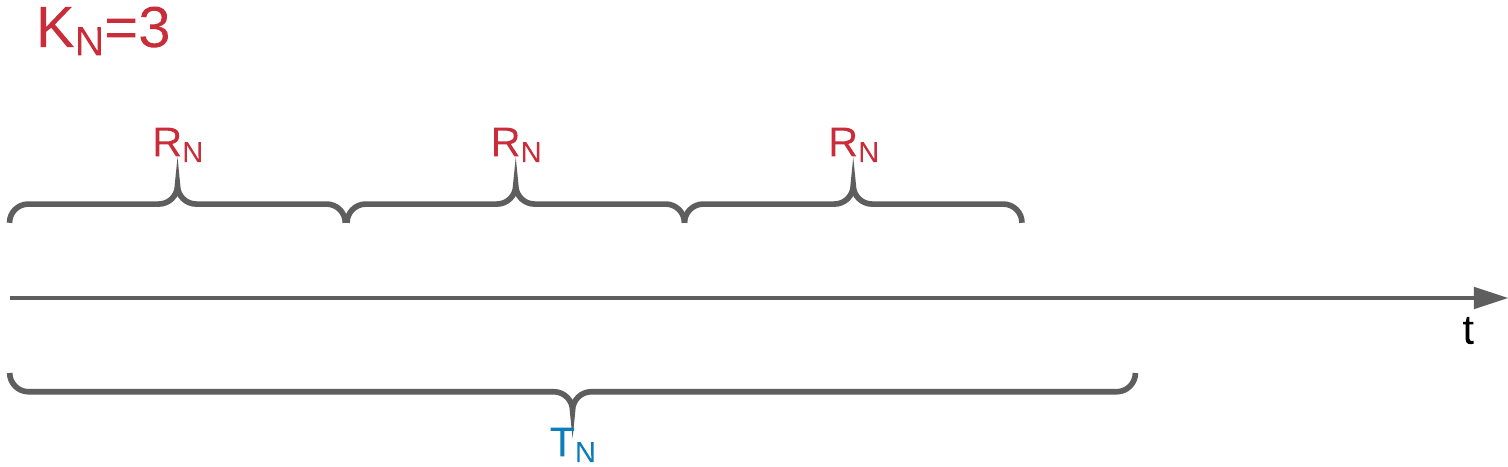
\includegraphics[scale=0.2]{./img/kn_rn.png}
        \caption{Example of $K_N$}
        \label{fig:kn_rn}
    \end{figure}
    Turns out that regardless of which of those intervals we choose for averaging, we can still make it highly probable that our temporal mean is as close to the $\mu(f)$ 
    as we want, given that we're free to increase $N$. 
\end{frame}

\begin{frame}
    In other words, we want to have a sequence $R_N$, such that:
    \begin{itemize}
        \item $R_N / \beta_N \rightarrow 0$ as $N \rightarrow \infty$
        \item for all $\varepsilon > 0$ and all observable quantities $f$
        \[
            \mathbb{P}\left[ \max_{\mathbb{N}_0 \ni k < K_N}|A_{R_N}(kR_N, f) - \mu(f)| < \varepsilon\right] \rightarrow 0
        \]
    \end{itemize}

    As $N \rightarrow \infty$. \\~\\
    Phew\ldots are we done now?
\end{frame}

\begin{frame}
    In other words, we want to have a sequence $R_N$, such that:
    \begin{itemize}
        \item $R_N / \beta_N \rightarrow 0$ as $N \rightarrow \infty$
        \item for all $\varepsilon > 0$ and all observable quantities $f$
        \[
            \mathbb{P}\left[ \max_{\mathbb{N}_0 \ni k < K_N}|A_{R_N}(kR_N, f) - \mu(f)| < \varepsilon\right] \rightarrow 0
        \]
    \end{itemize}

    As $N \rightarrow \infty$. \\~\\
    Phew\ldots are we done now? Not quite!
\end{frame}

\begin{frame}
    Turns out that we need the following technicality: we need to choose $L(\varepsilon, f) \in \mathbb{N}$, and we need to have that
    \begin{itemize}
        \item $L < N$
        \item $\Lambda(f) := supp(f) \subset [-N + L, N - L] \cap \mathbb{Z}$
    \end{itemize}
     Notice that $L$ does not depend on $N$. Thus, having to choose this $L$ doesn't restrict our choice of $f$ - it merely sets the minimum
     $N$ we can consider and we chose to grow $N \rightarrow \infty$.
    \\~\\
    We can partition the main interval as follows:
    \begin{itemize}
        \item $[-N, -N+L)$ - \textbf{left boundary region}
        \item $[-N+L, N-L]$ - \textbf{inside region}
        \item $(N-L, N]$ - \textbf{right boundary region}
    \end{itemize}

    \begin{figure}[H]
        \centering
        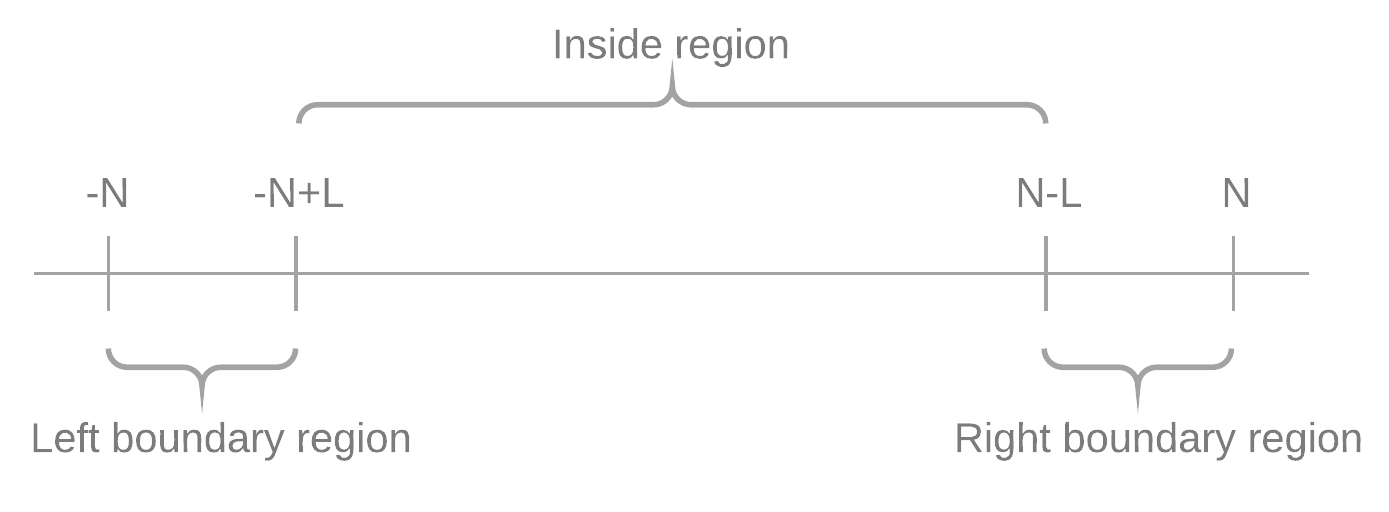
\includegraphics[scale=0.15]{./img/regions_df.png}
        \caption{Example of $K_N$}
        \label{fig:regions}
    \end{figure}
\end{frame}

\subsection{Statement of the theorem} % A subsection can be created just before a set of slides with a common theme to further break down your presentation into chunks

\begin{frame}
    \frametitle{Theorem 2}

    We're finally ready to formulate the theorem.

    \begin{theorem}[Thermalization]
        If $\lambda > \lambda^*$ there is a sequence $\{R_N\}_{N \in \mathbb{N}} \subset \mathbb{R_+}$ such that:
        \begin{itemize}
            \item $R_N/\beta_N \rightarrow 0$ as $N\rightarrow \infty$
            \item For all $\varepsilon > 0$ and observable quantities $f$ $\exists L(\varepsilon, f) \in \mathbb{N}$ such that
                  \[
                      \mathbb{P}\left[ \max_{\mathbb{N}_0 \ni k < K_N}|A_{R_N}(kR_N, f) - \mu(f)| > \varepsilon\right] \rightarrow 0
                  \]
                  as $N \rightarrow \infty$, where $K_N = \max\{k \in \mathbb{N}_0: kR_N < T_N\}$ and $\Lambda(f) \subset [-N + L, N - L] \cap \mathbb{Z}$
        \end{itemize}
    \end{theorem}
\end{frame}

\begin{frame}
    \frametitle{Proof}
    Set 
    \[B^N_k = \left\{ |A_{R_N}(kR_N, f) - \mu(f)| > \varepsilon\right\}\]
    On $B^N_k$ the difference between temporal mean of observalbe measured over the $k$-th interval and its expectation is greater than we'd like to.
    $B^N_k$~means \textbf{failure} (in $k$-th interval).
    \\~\\
    We want the probability of having no failures to go to 1
    \[\mathbb{P}\left[ \max_{\mathbb{N}_0 \ni k < K_N}|A_{R_N}(kR_N, f) - \mu(f)| \leq \varepsilon   \right] =
    \mathbb{P}\left[ \bigcap_{\mathbb{N}_0 \ni k < K_N}B_k^C \right] \rightarrow 1 \]
    as $N\rightarrow\infty$
\end{frame}

\begin{frame}
    \frametitle{Proof}
    It is easy to show that $\mathbb{P}(K_N = 0) \rightarrow 0$. Thus, we can safely focus only on the subset of $\Omega$ where $K_N \geq 1$. \\~\\
    Combining this with the event from the previous slide and applying some simple algebra, we arrive at the following bound
    \begin{align*}
        \mathbb{P}\left[ K_N \geq 1,  \bigcap_{\mathbb{N}_0 \ni k < K_N}B_k^C \right]
         \geq  \mathbb{P}[1 \leq K_N \leq m] - m^2\max_{1 \leq j}\max_{0 \leq k < j}\mathbb{P}\left[ B_k, K_{N} = j \right]
    \end{align*}
    Our objective will be to find a sequence $\{m_N\}_{N\in\mathbb{N}}$ such that:
    \begin{itemize}
        \item $\mathbb{P}[1 \leq K_N \leq m_N] \rightarrow 1$
        \item $m_N^2\max_{1 \leq j}\max_{0 \leq k < j}\mathbb{P}\left[ B_k, K_{N} = j \right] \rightarrow 0$ 
    \end{itemize}
    As $N \rightarrow \infty$
\end{frame}

\begin{frame}
    \frametitle{Proof}
    We will start with the second term. However, first we need some intermediate results. We will say $\xi_N(t)$ is \textbf{wide} at $t$ if 
    it intersects both boundary regions. In other words:
    \[
        \min\xi_N(t) < -N + L \land \max\xi_N(t) > N - L
    \]
    We will call the process \textbf{narrow} otherwise.
    \begin{figure}[H]
        \centering
        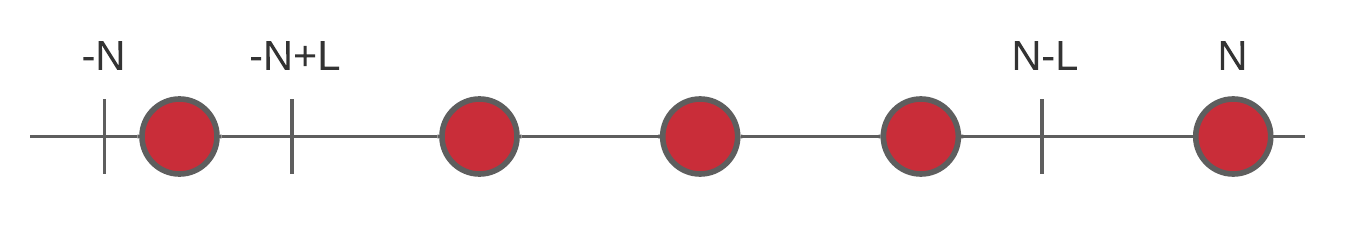
\includegraphics[scale=0.15]{./img/wide_process.png}
        \caption{Snapshot at $t$ of a process wide at $t$}
        \label{fig:wide_process}
    \end{figure}
    \begin{figure}[H]
        \centering
        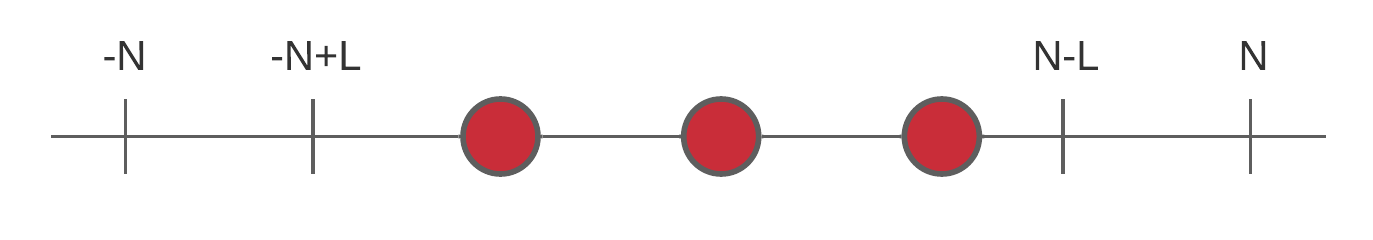
\includegraphics[scale=0.15]{./img/narrow_proces.png}
        \caption{Snapshot at $t$ of a process narrow at $t$}
        \label{fig:narrow_process}
    \end{figure}

\end{frame}
\begin{frame}
    \frametitle{Proof}
    \begin{lemma}[Shielding by a wide process]
        If $\xi_N(t)$ is wide at $t$, then \[\xi_N(t) = \xi(t)\text{ on }[-N + L, N - L] \cap \mathbb{Z}\]\\
        In particular we have $f(\xi_N(t)) = f(\xi(t))$
    \end{lemma}
    Why would this be true? \\~\\
\end{frame}

\begin{frame}
    Essentially, rightmost and leftmost infected individuals ``shield'' the entire space between them from outside influence.
    GIF SHOWING WHAT I MEAN
\end{frame}

\begin{frame}
    \frametitle{Proof}
    Define \[h_L(\eta) = I_{\{\xi : \xi \cup [-N, -N+L] = \varnothing\}}\]
    Notice that $h_L$ can tell us whether a process is wide or not.
    If we take $S$ to be a horizontal flip operator, then $h_L(\xi_N(t))h_L(S\xi_N(t))$ is the desired indicator.
    \begin{figure}[H]
        \centering
        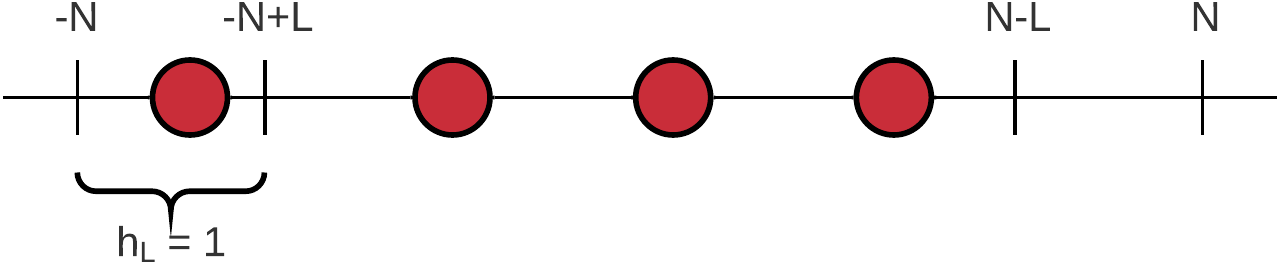
\includegraphics[scale=0.15]{./img/narrow_flip_ex_1.png}
        \caption{$h_L(\xi_N(t)) = 1$}
        \label{fig:narrow_flip_1}
    \end{figure}
    \begin{figure}[H]
        \centering
        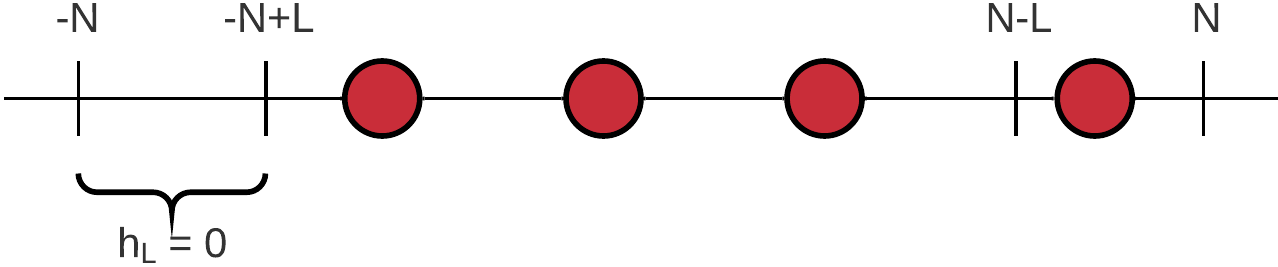
\includegraphics[scale=0.15]{./img/narrow_flip_ex_2.png}
        \caption{$h_L(S\xi_N(t)) = 0$}
        \label{fig:narrow_flip_2}
    \end{figure}

\end{frame}

\begin{frame}
    \begin{lemma}[Shielding of the left boundary region]
        \[\{T_N > t\} \subset \{h_L(\xi_N(t)) = h_L(\xi_{[-N, \infty)}(t))\}\]
    \end{lemma}
    In other words, if $\xi_N(t)$ is still alive, it fully determines whether $\xi_{[-N, \infty)}(t)$ intersects the left boundary region.
    \\~\\
    Why would this be true?
    \begin{itemize}
        \item If $\xi_N(t)$ intersects left boundary region, $\xi_{[-N, \infty)}$ intersects it too
        \item If $\xi_N(t)$ does not intersect the left boundary region, but has at least one node still alive, this node shields the left boundary region from outside influence.
            Moreover, no influence can propagate from $-N$. Hence, they need to agree on the left boundary region.
    \end{itemize}
\end{frame}

\begin{frame}
    GIF
\end{frame}

\begin{frame}
    \frametitle{Proof}
    Now we're ready to proceed. Recall, we want

    \begin{itemize}
        \item $m_N^2\max_{1 \leq j}\max_{0 \leq k < j}\mathbb{P}\left[ B_k, K_{N} = j \right] \rightarrow 0$ 
    \end{itemize}

    Let's take a closer look at $\mathbb{P}\left[ B_k, K_{N} = j \right]$. We will estimate the difference between the temporal average of $f(\xi_N)$ and it's expectation with 
    a triangle inequality.
    For $k < j$ we have

    \[
        \left|A_{R_N}(kR_N, f) - \mu(f)\right| > \varepsilon \rightarrow
    \]
    \begin{gather*}
        \rightarrow \left|R_N^{-1}\int_{kR_N}^{(k+1)R_N}f(\xi(t))dt - \mu(f)\right| > \varepsilon/2 \ \ \lor \\
        \left|R_N^{-1}\int_{kR_N}^{(k+1)R_N}f(\xi_N(t)) - f(\xi(t))dt \right| > \varepsilon/2
    \end{gather*}

\end{frame}

\begin{frame}
    \frametitle{Proof}
    Let's take the first term in the alternative and try to find a bound for

    \[
        \mathbb{P}\left[ \left|R_N^{-1}\int_{kR_N}^{(k+1)R_N}f(\xi(t))dt - \mu(f)\right| > \varepsilon/2 \right]
    \]

    It looks like we could almost apply weak convergence here, but we there's something missing\dots \\~\\ 
    Weak convergence to $\mu(f)$ as $R \rightarrow \infty$ holds for
    \[
        R_N^{-1}\int_{kR_N}^{(k+1)R_N}\mathbb{E}\left[ f(\xi(t)) \right]dt
    \]

    If we can now find a way to bind what's below, we're in business!
    \[
        \mathbb{P}\left[\left|R_N^{-1}\int_{kR_N}^{(k+1)R_N}f(\xi(t)) - \mathbb{E}\left[ f(\xi(t)) \right]dt > \varepsilon/4 \right|\right]
    \]
\end{frame}

\begin{frame}
    \frametitle{Proof}
    Turns out there is indeed a way to do that. This has to do with the fact that time correlations of $\xi(t)$ decay exponentially fast:
    \begin{theorem}[Exponentially decaying correlations]
        For any $f : \{0,1\}^\mathbb{Z}\rightarrow \mathbb{R}$ local, there are constants $C, \gamma$ such that 
        \[
            \left|\mathbb{C}ov\left[ f(\xi(t)), f(\xi(s))\right]\right| \leq Ce^{-\gamma|s-r|}
        \]
    \end{theorem}
    \visible<2->{
        Now, consider the variance of the expression from the previous slide:
        \[
            \mathbb{E}\left[  \left(R_N^{-1}\int_{kR_N}^{(k+1)R_N}f(\xi(t)) - \mathbb{E}\left[ f(\xi(t)) \right]dt \right)^2 \right]
        \]
    }
    \begin{itemize}
        \item<3-> Looks very much like we could get an expression for a covariance from this! 
        \item<4-> Then, Chebyshev will finish out our job for us.
    \end{itemize}
\end{frame}

\begin{frame}
    \frametitle{Proof}
    Recall, we've had:

    \begin{gather*}
        \mathbb{P}\left[ B_k, K_{N} = j \right] \leq \mathbb{P}\left[\left|R_N^{-1}\int_{kR_N}^{(k+1)R_N}f(\xi(t))dt - \mu(f)\right| > \varepsilon/2 \right] + \\
        \mathbb{P}\left[\left|R_N^{-1}\int_{kR_N}^{(k+1)R_N}f(\xi_N(t)) - f(\xi(t))dt \right| > \varepsilon/2\right]
    \end{gather*}

    We managed to bind the 1st term using:
    \begin{itemize}
        \item Weak convergence
        \item Exponentially decaying correlations + Chebyshev
    \end{itemize}

    Will this go through for the 2nd term?
    \begin{itemize}
        \item Weak convergence is a no-go. $\xi_N(t)$ converges weakly to $\delta_0$, but it does so at $\beta_N$ timescale, which is supposed to be large compared with $R_N$
    \end{itemize}
\end{frame}

\begin{frame}
    \frametitle{Proof}
    Let's massage the second term to see if we can get rid of $\xi_N$.

    \[
        \left|R_N^{-1}\int_{kR_N}^{(k+1)R_N}f(\xi_N(t)) - f(\xi(t))dt \right| > \varepsilon/2 
    \]

    Recall that 
    \begin{itemize}
        \item If $\xi_N$ is wide at $t$, we have $f(\xi_N(t)) = f(\xi(t))$ (shielding by a wide process). 
        \item We can use $h_L$ to tell whether a process is wide or not
        \item $\xi_N$ is alive for all $t$ we're considering. Hence $h_L(\xi_N(t)) = h_L(\xi_{[-N,\infty)}(t))$ (shielding of the left boundary region).
    \end{itemize}
    We get that the condition above implies

    \[
        2\norm{f}R_N^{-1}\int_{kR_N}^{(k+1)R_N}h_L(\xi_{[-N, \infty)}(t)) + h_L(S\xi_{(-\infty, N]}(t))dt > \varepsilon/2
    \]
\end{frame}


\begin{frame}
    \frametitle{Proof}
    By symmetry,
    \begin{gather*}
        \mathbb{P}\left[  2\norm{f}R_N^{-1}\int_{kR_N}^{(k+1)R_N}h_L(\xi_{[-N, \infty)}(t)) + h_L(S\xi_{(-\infty, N]}(t))dt > \varepsilon/2 \right] \leq \\
        2\mathbb{P}\left[ 2\norm{f}R_N^{-1}\int_{kR_N}^{(k+1)R_N}h_L(\xi_{[-N, \infty)}(t)) > \varepsilon/4 \right]
    \end{gather*}
    This form is something we could use the previous ``machinery'' (weak convergence + covariance + chebyshev) on, but:
    \begin{itemize}
        \item That method would us to make the time average arbitrarily close to $\mu(h_L)$, here we need to make it close to 0\dots
        \item Solution: make $\mu(h_L)$ close to 0! We can still vary $L$!
    \end{itemize}
\end{frame}

\begin{frame}
    \frametitle{Proof}
    Set $L$ to be such that 
    \[
        \mu_{[0, \infty)}\left( \left\{ A : A \cup [0,L] = \varnothing \right\} \right) \leq \varepsilon/16\norm{f}
    \]
    Notice how we have used that $\mu_{[0, \infty)}$ is translation invariant. Defining $L$ in this way makes it independent of $N$, as we wanted.
    Surprising, eh?
\end{frame}

\begin{frame}
    \frametitle{Proof}
    We've arrived at

    \[
        \mathbb{P}\left[ B^N_k, K_N = j \right] \leq \mathbb{P}\left[\Gamma_k^{R_N}\right] + 2\mathbb{P}\left[\tilde{\Gamma}_k^{R_N, L}\right]
    \]

    Where

    \[
        \Gamma_k^{R_N} := \left\{  \left|R_N^{-1}\int_{kR_N}^{(k+1)R_N}f(\xi(t))dt - \mu(f)\right| > \varepsilon/2\right\}
    \]

    \[
        \tilde{\Gamma}_k^{R_N} := \left\{  2\norm{f}R_N^{-1}\int_{kR_N}^{(k+1)R_N}h_L(\xi_{[-N, \infty)}(t)) > \varepsilon/4\right\}
    \]

    Formally, our previous considerations give us (for appropriate $R_N$, $L$)

    \[
        \mathbb{P}\left[ B^N_k, K_N = j \right] \leq \mathbb{P}\left[\Gamma_k^{R_N}\right] + 2\mathbb{P}\left[\tilde{\Gamma}_k^{R_N, L}\right] \leq C/R_N
    \]
\end{frame}

\begin{frame}
    \frametitle{Proof}
\end{frame}

%------------------------------------------------

\begin{frame}
\frametitle{Blocks of Highlighted Text}
\begin{block}{Block 1}
Lorem ipsum dolor sit amet, consectetur adipiscing elit. Integer lectus nisl, ultricies in feugiat rutrum, porttitor sit amet augue. Aliquam ut tortor mauris. Sed volutpat ante purus, quis accumsan dolor.
\end{block}

\begin{block}{Block 2}
Pellentesque sed tellus purus. Class aptent taciti sociosqu ad litora torquent per conubia nostra, per inceptos himenaeos. Vestibulum quis magna at risus dictum tempor eu vitae velit.
\end{block}

\begin{block}{Block 3}
Suspendisse tincidunt sagittis gravida. Curabitur condimentum, enim sed venenatis rutrum, ipsum neque consectetur orci, sed blandit justo nisi ac lacus.
\end{block}
\end{frame}

%------------------------------------------------

\begin{frame}
\frametitle{Multiple Columns}
\begin{columns}[c] % The "c" option specifies centered vertical alignment while the "t" option is used for top vertical alignment

\column{.45\textwidth} % Left column and width
\textbf{Heading}
\begin{enumerate}
\item Statement
\item Explanation
\item Example
\end{enumerate}

\column{.5\textwidth} % Right column and width
Lorem ipsum dolor sit amet, consectetur adipiscing elit. Integer lectus nisl, ultricies in feugiat rutrum, porttitor sit amet augue. Aliquam ut tortor mauris. Sed volutpat ante purus, quis accumsan dolor.

\end{columns}
\end{frame}

%------------------------------------------------
\section{Second Section}
%------------------------------------------------

\begin{frame}
\frametitle{Table}
\begin{table}
\begin{tabular}{l l l}
\toprule
\textbf{Treatments} & \textbf{Response 1} & \textbf{Response 2}\\
\midrule
Treatment 1 & 0.0003262 & 0.562 \\
Treatment 2 & 0.0015681 & 0.910 \\
Treatment 3 & 0.0009271 & 0.296 \\
\bottomrule
\end{tabular}
\caption{Table caption}
\end{table}
\end{frame}

%------------------------------------------------

\begin{frame}
\frametitle{Theorem}
\begin{theorem}[Mass--energy equivalence]
$E = mc^2$
\end{theorem}
\end{frame}

%------------------------------------------------

\begin{frame}[fragile] % Need to use the fragile option when verbatim is used in the slide
\frametitle{Verbatim}
\begin{example}[Theorem Slide Code]
\begin{verbatim}
\begin{frame}
\frametitle{Theorem}
\begin{theorem}[Mass--energy equivalence]
$E = mc^2$
\end{theorem}
\end{frame}\end{verbatim}
\end{example}
\end{frame}

%------------------------------------------------

\begin{frame}
\frametitle{Figure}
Uncomment the code on this slide to include your own image from the same directory as the template .TeX file.
%\begin{figure}
%\includegraphics[width=0.8\linewidth]{test}
%\end{figure}
\end{frame}

%------------------------------------------------

\begin{frame}[fragile] % Need to use the fragile option when verbatim is used in the slide
\frametitle{Citation}
An example of the \verb|\cite| command to cite within the presentation:\\~

This statement requires citation \cite{p1}.
\end{frame}

%------------------------------------------------

\begin{frame}
\frametitle{References}
\footnotesize{
\begin{thebibliography}{99} % Beamer does not support BibTeX so references must be inserted manually as below
\bibitem[Smith, 2012]{p1} John Smith (2012)
\newblock Title of the publication
\newblock \emph{Journal Name} 12(3), 45 -- 678.
\end{thebibliography}
}
\end{frame}

%------------------------------------------------

\begin{frame}
\Huge{\centerline{The End}}
\end{frame}

%----------------------------------------------------------------------------------------

\end{document} 
